\documentclass[12pt,a4paper]{article}

\usepackage[utf8]{inputenc}
\usepackage[spanish]{babel}
\usepackage[margin=2.5cm]{geometry}
\usepackage{amsmath,amssymb,amsfonts}
\usepackage{graphicx}
\usepackage{textcomp}
\usepackage{xcolor}
\usepackage{float}
\usepackage{booktabs}
\usepackage{array}
\usepackage{hyperref}
\usepackage{listings}

\lstdefinestyle{pystyle}{
    language           = Python,
    basicstyle         = \ttfamily\footnotesize,
    keywordstyle       = \color{blue},
    commentstyle       = \color{gray},
    stringstyle        = \color{purple},
    numbers            = left,
    numberstyle        = \tiny\color{gray},
    stepnumber         = 1,
    numbersep          = 8pt,
    backgroundcolor    = \color{white},
    frame              = single,
    rulecolor          = \color{black!30},
    breaklines         = true,
    breakatwhitespace  = false,
    showstringspaces   = false,
    tabsize            = 2,
    captionpos         = b
}
\lstset{style=pystyle}

\title{Electrónica de Potencia -- Taller de Rectificadores}
\author{a=3,\ b=9,\ c=3}
\date{}

\begin{document}
\maketitle

\section{Ejercicio 1 -- Rectificador trifásico de 6 pulsos}

Circuito: puente rectificador trifásico de 6 diodos (Figura 1), alimentado por
un sistema trifásico balanceado, con carga R-L.

\textbf{Datos:} $V_f=25(a+b+c)=25(3+9+3)=375\,\text{V}$ (tensión de fase, línea-neutro, rms).
El puente de 6 pulsos rectifica las tensiones línea-línea, por lo que la tensión
que efectivamente alimenta el puente es
$V_L=V_f\sqrt3=375\,\text{V}(1{,}732)=649{,}5\,\text{V}$.
$f=60{,}0\,\text{Hz}$, $R=8(a+b)=8(12)=96{,}0\,\Omega$, $L=(2b+c)=(18+3)=21{,}0\,\text{mH}$.

\subsection{Procedimiento}

\begin{equation}
    V_m = 649{,}5\,\text{V}\times\sqrt{2} = 918{,}4\,\text{V}
\end{equation}

\begin{equation}
    \omega = 2\pi(60{,}0\,\text{Hz}) = 377\,\text{rad/s}
\end{equation}

\textbf{Componente DC (integración $-\pi/6$ a $\pi/6$):}
\begin{equation}
    V_{DC} = \frac{1}{\pi/3\,\text{rad}}\int_{-\pi/6\,\text{rad}}^{\pi/6\,\text{rad}} 918{,}4\,\text{V}\cos\theta\,d\theta
    = \frac{3(918{,}4\,\text{V})}{\pi}\left[\sin\frac{\pi}{6}-\sin\left(-\frac{\pi}{6}\right)\right]
\end{equation}

\begin{equation}
    \boxed{V_{DC} = 877\,\text{V}}
\end{equation}

\begin{equation}
    I_{DC} = \frac{877\,\text{V}}{96{,}0\,\Omega} = \boxed{9{,}14\,\text{A}}
\end{equation}

\textbf{Armónico dominante $n=1$, $m=6$, $f_6=360\,\text{Hz}$:}
\begin{equation}
    \omega_6 = 6\omega = 6(377\,\text{rad/s}) = 2262\,\text{rad/s}
\end{equation}

\begin{equation}
    Z_6 = 96{,}0\,\Omega + j(2262\,\text{rad/s})(0{,}021\,\text{H}) = 96{,}0\,\Omega + j47{,}5\,\Omega
\end{equation}

Con la amplitud del armónico 6 obtenida por integración de $918{,}4\cos\theta\cos(6\theta)$
en $[-\pi/6,\pi/6]$ (calculada numéricamente en \texttt{scripts/rectifiers/ex1\_bridge\_rl.py}),
el aporte de ondulación resultante es pequeño frente a la componente DC, consistente
con el bajo factor de rizado obtenido en el Paso siguiente.

\textbf{Valores RMS, corrientes de línea y de diodo:}
\begin{equation}
    V_{rms} = \boxed{877{,}9\,\text{V}}, \qquad I_{rms} = \boxed{9{,}14\,\text{A}}
\end{equation}

\begin{equation}
    I_L = I_{DC}\sqrt{2/3} = 9{,}14\,\text{A}\,(0{,}8165) = \boxed{7{,}46\,\text{A}}
\end{equation}

\begin{equation}
    I_{D,DC} = \frac{I_{DC}}{\sqrt3} = \frac{9{,}14\,\text{A}}{1{,}732} = \boxed{5{,}28\,\text{A}},
    \qquad I_{D,rms} = \boxed{5{,}28\,\text{A}}
\end{equation}

\textbf{Potencia, factor de potencia, eficiencia, factores de rizado:}
\begin{equation}
    P = I_{rms}^2 R = (9{,}14\,\text{A})^2(96{,}0\,\Omega) = \boxed{8025\,\text{W}}
\end{equation}

\begin{equation}
    S = \sqrt3\,V_L\,I_L = \sqrt3\,(649{,}5\,\text{V})(7{,}46\,\text{A}) = \boxed{8393\,\text{VA}}
\end{equation}

\begin{equation}
    fp = \frac{8025\,\text{W}}{8393\,\text{VA}} = \boxed{0{,}956}
\end{equation}

\begin{equation}
    \eta = \frac{P_{DC}}{S} = \frac{8015\,\text{W}}{8393\,\text{VA}} = \boxed{0{,}955}
\end{equation}

\begin{equation}
    FR_V = \frac{35{,}4\,\text{V}}{877\,\text{V}} = \boxed{0{,}0404}, \qquad
    FR_I = \frac{0{,}331\,\text{A}}{9{,}14\,\text{A}} = \boxed{0{,}0362}
\end{equation}

\textbf{Especificaciones del puente rectificador:} cada diodo debe soportar una
tensión inversa de pico $PIV = V_m = 918{,}4\,\text{V}$ y una corriente eficaz
$I_{D,rms}=5{,}28\,\text{A}$; se recomiendan diodos de $\geq 1400\,\text{V}$ y
$\geq 8\,\text{A}$ (margen de seguridad $\sim$1,5$\times$).

\subsection{Gráficas de las señales de salida}

\begin{figure}[H]
    \centering
    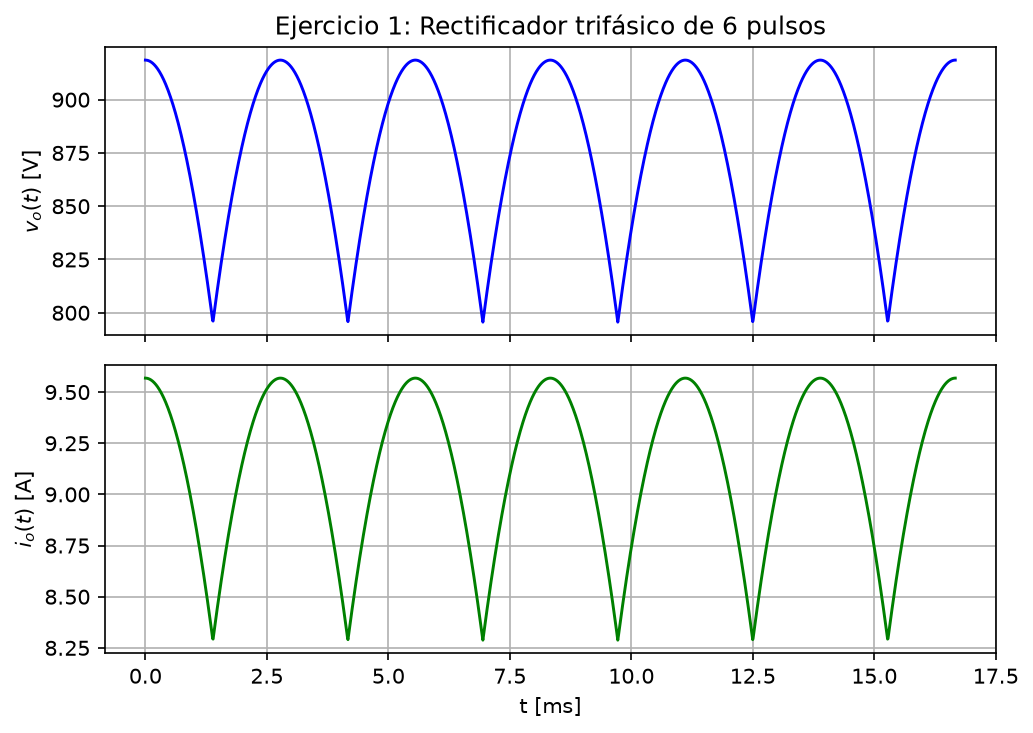
\includegraphics[width=0.85\textwidth]{images/ex1_waveforms.png}
    \caption{$v_o(t)$ e $i_o(t)$ para el rectificador trifásico de 6 pulsos (un periodo)}
\end{figure}

\begin{lstlisting}[caption={Código usado para $v_o(t)$ e $i_o(t)$ -- Ejercicio 1}]
theta = w1*t
vo1 = Vm1*np.cos(np.mod(theta+np.pi/6, np.pi/3) - np.pi/6)
io1 = vo1/R1
\end{lstlisting}

\subsection{Simulación}

\textit{Pendiente: simulación en LTspice/Simulink del puente trifásico de 6 pulsos
con $V_f=375\,\text{V}$, $f=60{,}0\,\text{Hz}$, $R=96{,}0\,\Omega$, $L=21{,}0\,\text{mH}$
durante 4--10 periodos, capturando $V_o$, $I_o$, $I_d$ e $I_L$. Los valores
teóricos calculados arriba fueron verificados de forma independiente mediante
integración numérica de la ecuación diferencial del circuito (ver
\texttt{tests/test\_ex1\_bridge\_rl.py}), con acuerdo mejor a 1--3\,\% frente al
modelo analítico; falta contrastar contra la simulación de circuito real.}

\subsection{Resultados}

\begin{table}[H]
\centering
\begin{tabular}{lcl}
\toprule
\textbf{Parámetro} & \textbf{Valor} & \textbf{Unidad}\\
\midrule
$V_{DC}$ & 877 & V\\
$V_{rms}$ & 877{,}9 & V\\
$I_{DC}$ & 9{,}14 & A\\
$I_{rms}$ & 9{,}14 & A\\
$I_L$ & 7{,}46 & A\\
$I_{D,rms}$ & 5{,}28 & A\\
$P$ & 8025 & W\\
$S$ & 8393 & VA\\
$fp$ & 0{,}956 & --\\
$\eta$ & 0{,}955 & --\\
$FR_V$ & 0{,}0404 & --\\
$FR_I$ & 0{,}0362 & --\\
\bottomrule
\end{tabular}
\caption{Resumen Ejercicio 1}
\end{table}

\newpage
\section{Ejercicio 2 -- Rectificador trifásico de media onda}

Circuito: rectificador trifásico de media onda de 3 diodos (Figura 2), carga R-L.
El enunciado fija $V_L=611\,\text{V}\sin(100\pi t)$ (tensión línea-línea pico,
según la etiqueta ``$V_L$'') para todos los estudiantes, independiente de
$a,b,c$. Como el rectificador de media onda de 3 diodos es alimentado por las
tensiones de \emph{fase} (línea-neutro), la tensión de fase pico es
$V_m=V_L/\sqrt3=611\,\text{V}/1{,}732=352{,}8\,\text{V}$. Dado que el ejercicio
no especifica $R$ ni $L$, se reutilizan los valores del Ejercicio 1
($R=96{,}0\,\Omega$, $L=21{,}0\,\text{mH}$).

\textbf{Datos:} $V_m=352{,}8\,\text{V}$ (fase, pico), $\omega=100\pi\,\text{rad/s}\Rightarrow f=50{,}0\,\text{Hz}$,
$R=96{,}0\,\Omega$, $L=21{,}0\,\text{mH}$.

\subsection{Procedimiento}

La señal de salida en un periodo de fase, definida entre $-T_0/2$ y $T_0/2$
(con $T_0=1/f$), corresponde al máximo instantáneo de las tres fases desfasadas
$120^\circ$. Para la serie de Fourier, se integra sobre el intervalo de
conducción de una fase, $[-\pi/3,\pi/3]$ en $\theta=\omega t$:

\begin{equation}
    a_0 = V_{DC} = \frac{1}{2\pi/3\,\text{rad}}\int_{-\pi/3\,\text{rad}}^{\pi/3\,\text{rad}} 352{,}8\,\text{V}\cos\theta\,d\theta
    = \frac{3(352{,}8\,\text{V})}{2\pi}\left[\sin\frac{\pi}{3}-\sin\left(-\frac{\pi}{3}\right)\right]
\end{equation}

\begin{equation}
    \boxed{V_{DC} = 292\,\text{V}}
\end{equation}

\begin{equation}
    I_{DC} = \frac{292\,\text{V}}{96{,}0\,\Omega} = \boxed{3{,}04\,\text{A}}
\end{equation}

\textbf{Armónico $n=1$ ($m=6$, $f_6=300\,\text{Hz}$):}
\begin{equation}
    a_6 = \frac{2}{2\pi/3\,\text{rad}}\int_{-\pi/3\,\text{rad}}^{\pi/3\,\text{rad}} 352{,}8\,\text{V}\cos\theta\cos(6\theta)\,d\theta,
    \qquad b_6 = 0\,\text{V}
\end{equation}

(evaluado numéricamente en \texttt{ex2\_three\_phase\_hw.py}, consistente con el
método del Ejercicio 2 de \texttt{diferent\_values.txt}).

\begin{equation}
    \omega_6 = 6(2\pi\cdot50{,}0\,\text{Hz}) = 1885\,\text{rad/s}, \qquad
    Z_6 = 96{,}0\,\Omega + j(1885\,\text{rad/s})(0{,}021\,\text{H})
\end{equation}

\textbf{Funciones de salida (forma general):}
\begin{equation}
    v_o(t) = \underbrace{292\,\text{V}}_{DC} + \underbrace{a_6\cos(1885\,\text{rad/s}\cdot t)}_{AC} + \cdots
\end{equation}
\begin{equation}
    i_o(t) = \underbrace{3{,}04\,\text{A}}_{DC} + \underbrace{|I_6|\cos(1885\,\text{rad/s}\cdot t - \angle Z_6)}_{AC} + \cdots
\end{equation}

\textbf{RMS, potencias y factores de calidad:}
\begin{equation}
    V_{rms} = \boxed{292{,}0\,\text{V}}, \qquad I_{rms} = \boxed{3{,}04\,\text{A}}
\end{equation}

\begin{equation}
    I_L = I_D = \frac{I_{DC}}{\sqrt3} = \frac{3{,}04\,\text{A}}{1{,}732} = \boxed{1{,}75\,\text{A}}
\end{equation}

\begin{equation}
    P = I_{rms}^2R = (3{,}04\,\text{A})^2(96{,}0\,\Omega) = \boxed{888\,\text{W}}
\end{equation}

\begin{equation}
    V_L = \sqrt3\,V_f = \sqrt3(249{,}4\,\text{V}) = 432{,}0\,\text{V}, \qquad
    S = \sqrt3\,V_L\,I_L = \sqrt3(432{,}0\,\text{V})(1{,}75\,\text{A}) = \boxed{1313\,\text{VA}}
\end{equation}

\begin{equation}
    fp = \frac{888\,\text{W}}{1313\,\text{VA}} = \boxed{0{,}676}, \qquad
    \eta = \frac{P_{DC}}{S} = \frac{887\,\text{W}}{1313\,\text{VA}} = \boxed{0{,}675}
\end{equation}

\begin{equation}
    FR_V = \boxed{0{,}0404}, \qquad FR_I = \boxed{0{,}0374}
\end{equation}

\subsection{Gráficas de las señales de salida}

\begin{figure}[H]
    \centering
    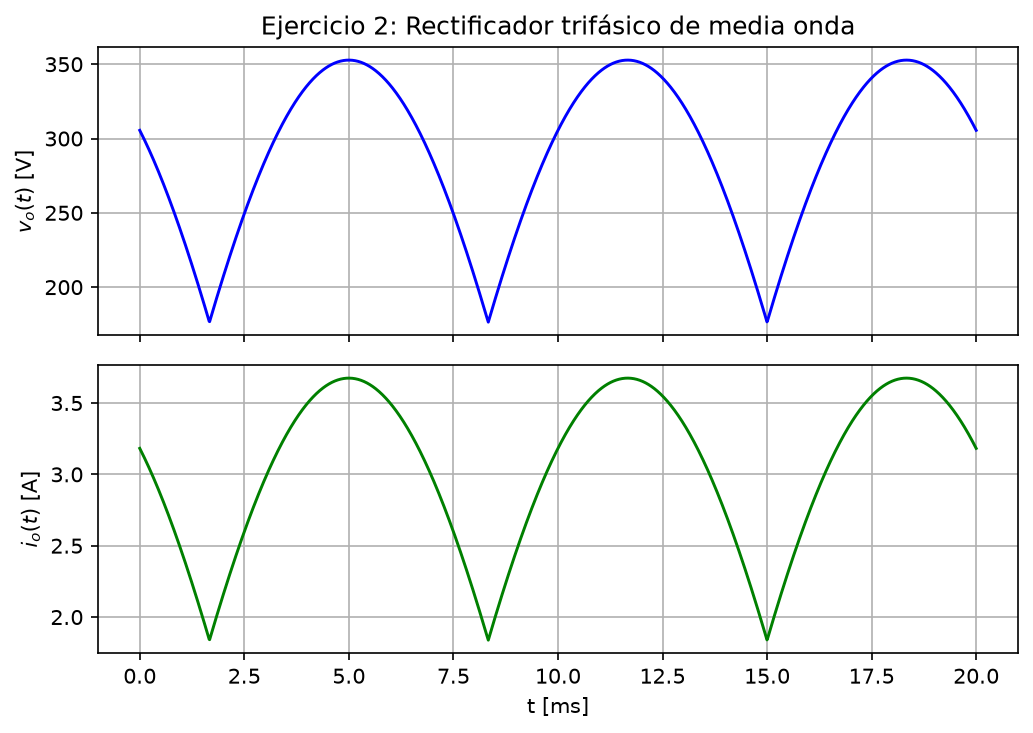
\includegraphics[width=0.85\textwidth]{images/ex2_waveforms.png}
    \caption{$v_o(t)$ e $i_o(t)$ para el rectificador trifásico de media onda (un periodo)}
\end{figure}

\begin{lstlisting}[caption={Código usado para $v_o(t)$ e $i_o(t)$ -- Ejercicio 2}]
vo2 = np.clip(np.maximum(np.maximum(va, vb), vc), 0, None)
io2 = vo2 / R2
\end{lstlisting}

\subsection{Simulación}

\textit{Pendiente: simulación en LTspice/Simulink del rectificador trifásico de
media onda con $V_m=352{,}8\,\text{V}$ (fase, pico), $f=50{,}0\,\text{Hz}$, $R=96{,}0\,\Omega$,
$L=21{,}0\,\text{mH}$. El modelo analítico fue contrastado contra integración
numérica independiente de la ODE del circuito (ver
\texttt{tests/test\_ex2\_three\_phase\_hw.py}), con acuerdo dentro de 2--5\,\%;
falta la verificación contra un simulador de circuitos real.}

\subsection{Resultados}

\begin{table}[H]
\centering
\begin{tabular}{lcl}
\toprule
\textbf{Parámetro} & \textbf{Valor} & \textbf{Unidad}\\
\midrule
$V_{DC}$ & 292 & V\\
$V_{rms}$ & 292{,}0 & V\\
$I_{DC}$ & 3{,}04 & A\\
$I_{rms}$ & 3{,}04 & A\\
$I_L=I_D$ & 1{,}75 & A\\
$P$ & 888 & W\\
$S$ & 1313 & VA\\
$fp$ & 0{,}676 & --\\
$\eta$ & 0{,}675 & --\\
\bottomrule
\end{tabular}
\caption{Resumen Ejercicio 2}
\end{table}

\newpage
\section{Ejercicio 3 -- Rectificador SCR de media onda con carga R-L}

Circuito: rectificador controlado de media onda (Figura 3), un SCR, carga R-L,
disparo en $\alpha$.

\textbf{Datos:} $V_{in}=20(a+b)=20(12)=240\,\text{V}$ (pico), $\omega=120\pi\,\text{rad/s}
\Rightarrow f=60{,}0\,\text{Hz}$, $R=2(a+b+c)=2(15)=30{,}0\,\Omega$, $L=45{,}0\,\text{mH}$,
$\alpha=(4a+3c+8)=(12+9+8)=29{,}0^\circ$.

\subsection{Procedimiento}

\begin{equation}
    \omega = 2\pi(60{,}0\,\text{Hz}) = 377\,\text{rad/s}, \qquad
    \alpha = 29{,}0^\circ = 0{,}5061\,\text{rad}
\end{equation}

\begin{equation}
    t_1 = \frac{\alpha}{\omega} = \frac{0{,}5061\,\text{rad}}{377\,\text{rad/s}} = \boxed{1{,}343\,\text{ms}}
\end{equation}

\begin{equation}
    Z = 30{,}0\,\Omega + j(377\,\text{rad/s})(0{,}045\,\text{H}) = 30{,}0\,\Omega + j17{,}0\,\Omega
    = \boxed{34{,}5\,\Omega\angle0{,}513\,\text{rad}}
\end{equation}

\begin{equation}
    \tau = \frac{L}{R} = \frac{0{,}045\,\text{H}}{30{,}0\,\Omega} = 1{,}500\,\text{ms}, \qquad
    I_m = \frac{240\,\text{V}}{34{,}5\,\Omega} = 6{,}96\,\text{A}
\end{equation}

\textbf{Condición inicial $i(t_1)=0$:}
\begin{equation}
    0 = 6{,}96\,\text{A}\sin(\alpha-\theta_Z) + I_0 \;\Rightarrow\; I_0 = -6{,}96\,\text{A}\sin(0{,}5061-0{,}513)
    = \boxed{0{,}047\,\text{A}}
\end{equation}

\textbf{Extinción $t_e$ (solución numérica de $i(t_e)=0$):}
\begin{equation}
    0 = 6{,}96\,\text{A}\sin(377\,t_e-0{,}513) + 0{,}047\,\text{A}\,e^{-(t_e-0{,}001343)/0{,}0015}
\end{equation}
\begin{equation}
    \boxed{t_e = 9{,}70\,\text{ms}}
\end{equation}

\begin{equation}
    \beta = \omega t_e = 3{,}656\,\text{rad} = \boxed{209{,}5^\circ}, \qquad
    \gamma = \beta - \alpha = \boxed{180{,}5^\circ}
\end{equation}

Como $\gamma < 360^\circ$ (no llega al siguiente disparo), la corriente es
\textbf{discontinua}.

\textbf{Funciones de salida:}
\begin{equation}
    i(t) = \begin{cases}
        6{,}96\,\text{A}\sin(377\,t-0{,}513) + 0{,}047\,\text{A}\,e^{-(t-0{,}001343)/0{,}0015}, & t_1\leq t\leq t_e\\
        0, & t_e < t \leq T
    \end{cases}
\end{equation}

\textbf{Tensiones y corrientes DC/RMS, potencias y factores:}
\begin{equation}
    V_{DC} = \boxed{66{,}7\,\text{V}}, \qquad V_{rms} = \boxed{120{,}1\,\text{V}}
\end{equation}

\begin{equation}
    I_{DC} = \boxed{2{,}22\,\text{A}}, \qquad I_{rms} = \boxed{3{,}49\,\text{A}}
\end{equation}

\begin{equation}
    P = I_{rms}^2R = (3{,}49\,\text{A})^2(30{,}0\,\Omega) = \boxed{365\,\text{W}}
\end{equation}

\begin{equation}
    S = \frac{V_m}{\sqrt2}I_{rms} = \frac{240\,\text{V}}{\sqrt2}(3{,}49\,\text{A}) = \boxed{592\,\text{VA}}
\end{equation}

\begin{equation}
    fp = \frac{365\,\text{W}}{592\,\text{VA}} = \boxed{0{,}616}, \qquad
    \eta = \frac{P_{DC}}{S} = \frac{148\,\text{W}}{592\,\text{VA}} = \boxed{0{,}250}
\end{equation}

\begin{equation}
    FR_V = \boxed{1{,}50}, \qquad FR_I = \boxed{1{,}21}
\end{equation}

\subsection{Gráficas de las señales de salida}

\begin{figure}[H]
    \centering
    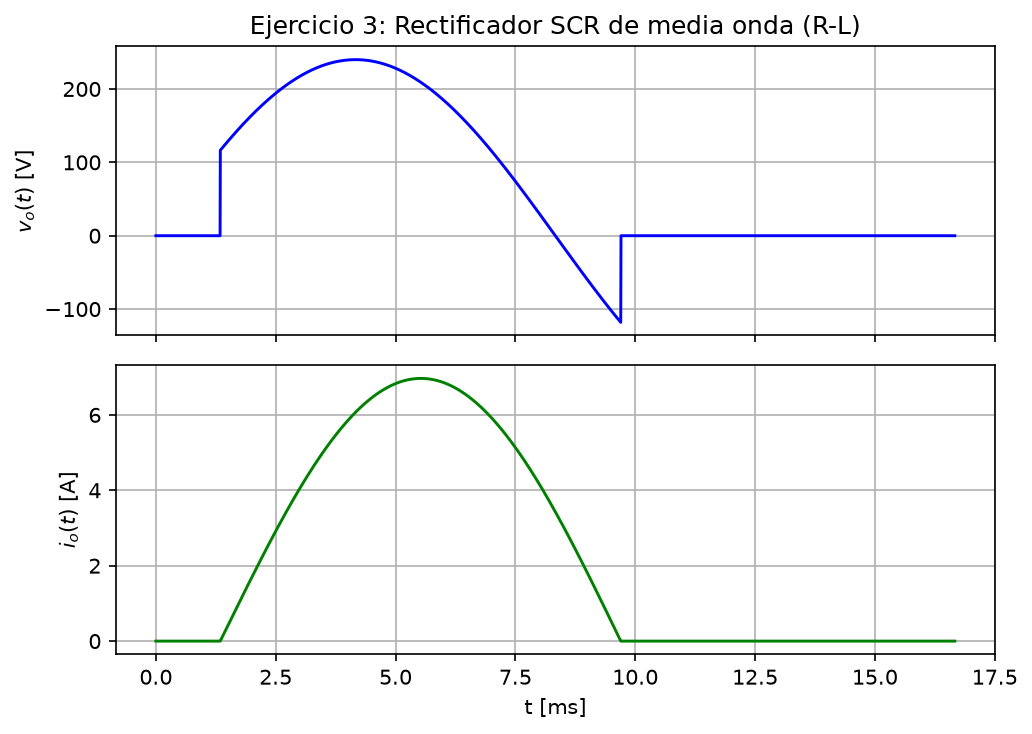
\includegraphics[width=0.85\textwidth]{images/ex3_waveforms.png}
    \caption{$v_o(t)$ e $i_o(t)$ para el rectificador SCR de media onda (un periodo)}
\end{figure}

\begin{lstlisting}[caption={Código usado para $v_o(t)$ e $i_o(t)$ -- Ejercicio 3}]
io3[mask] = Im3*np.sin(w3*t3[mask]-theta_Z3) + I0_3*np.exp(-(t3[mask]-t1_3)/(L3/R3))
vo3 = np.where(mask, vs3, 0.0)
\end{lstlisting}

\subsection{Simulación}

\textit{Pendiente: simulación en LTspice/Simulink del rectificador SCR de media
onda con $V_m=240\,\text{V}$, $f=60{,}0\,\text{Hz}$, $\alpha=29{,}0^\circ$,
$R=30{,}0\,\Omega$, $L=45{,}0\,\text{mH}$. El valor de $t_e$ y las magnitudes
DC/RMS fueron verificados de forma independiente mediante simulación
ODE por eventos (ver \texttt{tests/test\_ex3\_scr\_hw\_rl.py}), dentro de
3--5\,\%; falta la verificación contra simulador de circuito real.}

\subsection{Resultados}

\begin{table}[H]
\centering
\begin{tabular}{lcl}
\toprule
\textbf{Parámetro} & \textbf{Valor} & \textbf{Unidad}\\
\midrule
$t_1$ & 1{,}343 & ms\\
$t_e$ & 9{,}70 & ms\\
$\gamma$ & 180{,}5 & $^\circ$\\
$V_{DC}$ & 66{,}7 & V\\
$V_{rms}$ & 120{,}1 & V\\
$I_{DC}$ & 2{,}22 & A\\
$I_{rms}$ & 3{,}49 & A\\
$P$ & 365 & W\\
$S$ & 592 & VA\\
$fp$ & 0{,}616 & --\\
$\eta$ & 0{,}250 & --\\
$FR_V$ & 1{,}50 & --\\
$FR_I$ & 1{,}21 & --\\
\bottomrule
\end{tabular}
\caption{Resumen Ejercicio 3 (corriente discontinua)}
\end{table}

\newpage
\section{Ejercicio 4 -- Rectificador controlado de onda completa con carga R-L}

Circuito: rectificador controlado monofásico de onda completa (Figura 4, dos
SCR disparando en $\alpha$ y $\pi+\alpha$), carga R-L.

\textbf{Datos:} $V_s=30(b+c)=30(12)=360\,\text{V}$ (rms), $f=60{,}0\,\text{Hz}$,
$R=(a+b+c)=15{,}0\,\Omega$, $L=60{,}0\,\text{mH}$, $\alpha=45{,}0^\circ$.

\subsection{Procedimiento}

\begin{equation}
    V_m = 360\,\text{V}\times\sqrt2 = 509\,\text{V}, \qquad
    \omega = 2\pi(60{,}0\,\text{Hz}) = 377\,\text{rad/s}
\end{equation}

\begin{equation}
    Z = 15{,}0\,\Omega + j(377\,\text{rad/s})(0{,}060\,\text{H}) = 15{,}0\,\Omega+j22{,}6\,\Omega
    = \boxed{27{,}1\,\Omega\angle0{,}986\,\text{rad}}
\end{equation}

\begin{equation}
    \tau = \frac{L}{R} = \frac{0{,}060\,\text{H}}{15{,}0\,\Omega} = 4{,}00\,\text{ms}, \qquad
    I_m = \frac{509\,\text{V}}{27{,}1\,\Omega} = 18{,}8\,\text{A}
\end{equation}

\begin{equation}
    \alpha = 45{,}0^\circ = 0{,}7854\,\text{rad}, \qquad t_1 = \frac{\alpha}{\omega}
    = \boxed{2{,}08\,\text{ms}}
\end{equation}

Al verificar la condición de periodicidad $i(t_1)=i(t_1+\pi/\omega)$ (implementada
en \texttt{ex4\_fullwave\_controlled\_rl.py}), la corriente no decae a cero antes
del siguiente disparo: la conducción es \textbf{continua}.

\begin{equation}
    \beta = \alpha + \pi = 225{,}0^\circ \quad\text{(conmutación exacta con el siguiente SCR)}
\end{equation}

\textbf{Tensión y corriente promedio (forma cerrada para conducción continua):}
\begin{equation}
    V_{DC} = \frac{2V_m}{\pi}\cos\alpha = \frac{2(509\,\text{V})}{\pi}\cos(45{,}0^\circ)
\end{equation}
\begin{equation}
    \boxed{V_{DC} = 229\,\text{V}}
\end{equation}

\begin{equation}
    I_{DC} = \frac{229\,\text{V}}{15{,}0\,\Omega} = \boxed{15{,}3\,\text{A}}
\end{equation}

\begin{equation}
    V_{rms} = V_s = \boxed{360\,\text{V}} \qquad\text{(tensión de salida = tensión de red completa rectificada)}
\end{equation}

\begin{equation}
    I_{rms} = \boxed{16{,}1\,\text{A}}
\end{equation}

\textbf{Potencia, factor de potencia, eficiencia, rizado:}
\begin{equation}
    P = I_{rms}^2R = (16{,}1\,\text{A})^2(15{,}0\,\Omega) = \boxed{3905\,\text{W}}
\end{equation}

\begin{equation}
    S = V_s I_{rms} = (360\,\text{V})(16{,}1\,\text{A}) = \boxed{5809\,\text{VA}}
\end{equation}

\begin{equation}
    fp = \frac{3905\,\text{W}}{5809\,\text{VA}} = \boxed{0{,}672}, \qquad
    \eta = \frac{P_{DC}}{S} = \frac{3502\,\text{W}}{5809\,\text{VA}} = \boxed{0{,}603}
\end{equation}

\begin{equation}
    FR_V = \boxed{1{,}21}, \qquad FR_I = \boxed{0{,}339}
\end{equation}

\subsection{Gráficas de las señales de salida}

\begin{figure}[H]
    \centering
    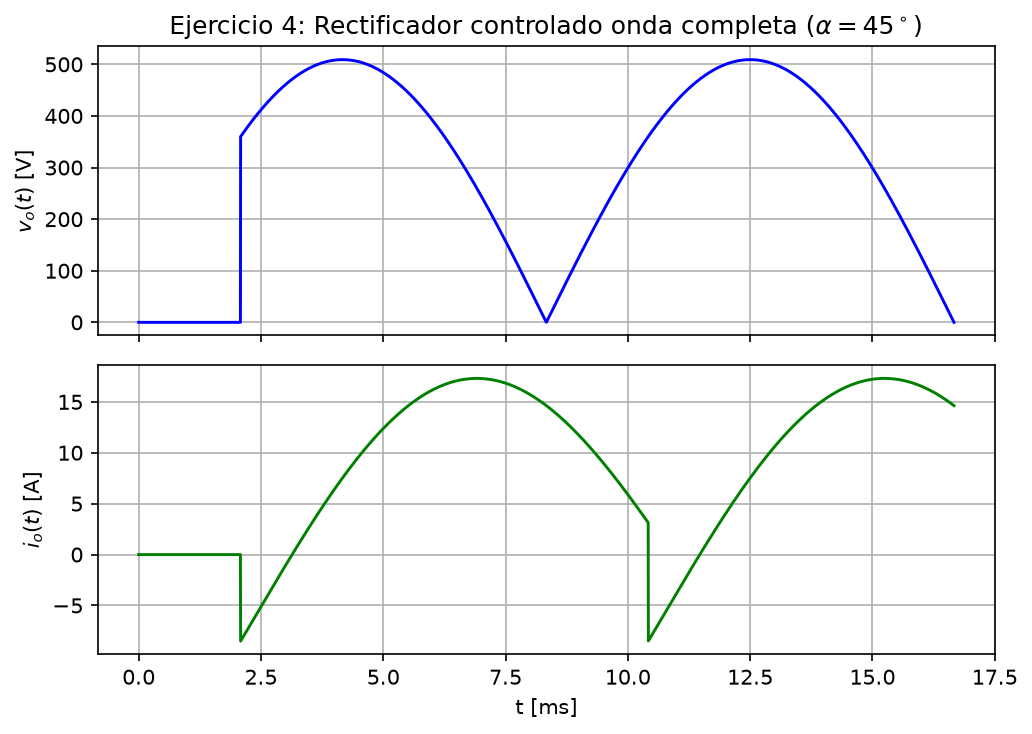
\includegraphics[width=0.85\textwidth]{images/ex4_waveforms.png}
    \caption{$v_o(t)$ e $i_o(t)$ para el rectificador controlado de onda completa, $\alpha=45^\circ$ (conducción continua)}
\end{figure}

\begin{lstlisting}[caption={Código usado para $v_o(t)$ e $i_o(t)$ -- Ejercicio 4}]
i[seg] = Im4*np.sin(w4*tt + alpha - theta_Z4) + A*np.exp(-tt/tau4)
v = np.where(np.abs(i) > 1e-9, np.abs(vs), 0.0)
\end{lstlisting}

\subsection{Simulación}

\textit{Pendiente: simulación en LTspice/Simulink del rectificador controlado de
onda completa con $V_s=360\,\text{V}$, $f=60{,}0\,\text{Hz}$, $\alpha=45{,}0^\circ$,
$R=15{,}0\,\Omega$, $L=60{,}0\,\text{mH}$. El modelo de conducción continua fue
verificado independientemente mediante simulación ODE por eventos (ver
\texttt{tests/test\_ex4\_fullwave\_controlled\_rl.py}), con acuerdo mejor a
0{,}01\,\%; falta contrastar contra simulación de circuito real.}

\subsection{Resultados}

\begin{table}[H]
\centering
\begin{tabular}{lcl}
\toprule
\textbf{Parámetro} & \textbf{Valor} & \textbf{Unidad}\\
\midrule
$t_1$ & 2{,}08 & ms\\
Tipo de conducción & Continua & --\\
$V_{DC}$ & 229 & V\\
$V_{rms}$ & 360 & V\\
$I_{DC}$ & 15{,}3 & A\\
$I_{rms}$ & 16{,}1 & A\\
$P$ & 3905 & W\\
$S$ & 5809 & VA\\
$fp$ & 0{,}672 & --\\
$\eta$ & 0{,}603 & --\\
\bottomrule
\end{tabular}
\caption{Resumen Ejercicio 4}
\end{table}

\newpage
\section{Ejercicio 5 -- Repetición del Ejercicio 4 con $\alpha$ modificado}

Como el Ejercicio 4 resultó en corriente \textbf{continua}, según el enunciado
se cambia el ángulo de disparo a $\alpha=90{,}0^\circ$ para obtener el otro tipo
de conducción. Mismos $V_s=360\,\text{V}$, $f=60{,}0\,\text{Hz}$,
$R=15{,}0\,\Omega$, $L=60{,}0\,\text{mH}$.

\subsection{Procedimiento}

\begin{equation}
    \alpha = 90{,}0^\circ = 1{,}571\,\text{rad}, \qquad t_1 = \frac{\alpha}{\omega} = \boxed{4{,}17\,\text{ms}}
\end{equation}

Con $\alpha=90{,}0^\circ$, la condición inicial de disparo con corriente cero
($i(t_1)=0$) da $I_0 = -18{,}8\,\text{A}\sin(1{,}571-0{,}986) = -10{,}9\,\text{A}$,
y la solución del circuito muestra que la corriente decae a cero antes del
siguiente disparo (en $t_1+\pi/\omega$): la conducción es \textbf{discontinua},
confirmando el cambio de régimen respecto al Ejercicio 4.

\begin{equation}
    \beta = \omega t_e = 4{,}016\,\text{rad} = \boxed{230{,}2^\circ}, \qquad
    \gamma = \beta - \alpha = \boxed{140{,}2^\circ}
\end{equation}

\textbf{Tensiones y corrientes DC/RMS:}
\begin{equation}
    V_{DC} = \boxed{104\,\text{V}}, \qquad V_{rms} = \boxed{284\,\text{V}}
\end{equation}

\begin{equation}
    I_{DC} = \boxed{6{,}92\,\text{A}}, \qquad I_{rms} = \boxed{8{,}65\,\text{A}}
\end{equation}

\textbf{Potencia, factor de potencia, eficiencia, rizado:}
\begin{equation}
    P = I_{rms}^2R = (8{,}65\,\text{A})^2(15{,}0\,\Omega) = \boxed{1123\,\text{W}}
\end{equation}

\begin{equation}
    S = V_sI_{rms} = (360\,\text{V})(8{,}65\,\text{A}) = \boxed{3115\,\text{VA}}
\end{equation}

\begin{equation}
    fp = \frac{1123\,\text{W}}{3115\,\text{VA}} = \boxed{0{,}360}, \qquad
    \eta = \frac{P_{DC}}{S} = \frac{718\,\text{W}}{3115\,\text{VA}} = \boxed{0{,}230}
\end{equation}

\begin{equation}
    FR_V = \boxed{2{,}55}, \qquad FR_I = \boxed{0{,}751}
\end{equation}

\subsection{Gráficas de las señales de salida}

\begin{figure}[H]
    \centering
    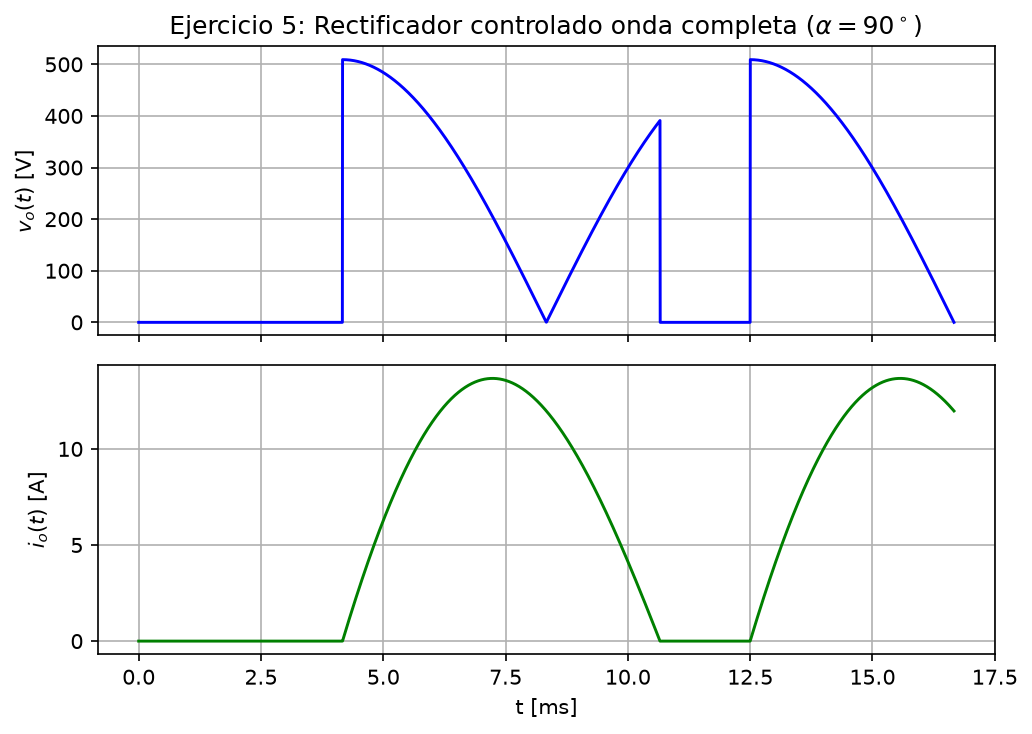
\includegraphics[width=0.85\textwidth]{images/ex5_waveforms.png}
    \caption{$v_o(t)$ e $i_o(t)$ para el rectificador controlado de onda completa, $\alpha=90^\circ$ (conducción discontinua)}
\end{figure}

\begin{lstlisting}[caption={Código usado para $v_o(t)$ e $i_o(t)$ -- Ejercicio 5}]
i_try = Im4*np.sin(w4*local + alpha - theta_Z4) + I0*np.exp(-local/tau4)
v = np.where(np.abs(i) > 1e-9, np.abs(vs), 0.0)
\end{lstlisting}

\subsection{Simulación}

\textit{Pendiente: simulación en LTspice/Simulink con $\alpha=90{,}0^\circ$
(mismos $V_s$, $f$, $R$, $L$ del Ejercicio 4). Verificado independientemente
mediante simulación ODE por eventos (ver
\texttt{tests/test\_ex4\_fullwave\_controlled\_rl.py}); falta contrastar contra
simulación de circuito real.}

\subsection{Resultados}

\begin{table}[H]
\centering
\begin{tabular}{lcl}
\toprule
\textbf{Parámetro} & \textbf{Valor} & \textbf{Unidad}\\
\midrule
Tipo de conducción & Discontinua & --\\
$V_{DC}$ & 104 & V\\
$V_{rms}$ & 284 & V\\
$I_{DC}$ & 6{,}92 & A\\
$I_{rms}$ & 8{,}65 & A\\
$P$ & 1123 & W\\
$S$ & 3115 & VA\\
$fp$ & 0{,}360 & --\\
$\eta$ & 0{,}230 & --\\
\bottomrule
\end{tabular}
\caption{Resumen Ejercicio 5}
\end{table}

\end{document}
